\subsection{Diskussion}

Ziel dieser Bachelorarbeit war es, die Serverless Architektur zu betrachten, und nach einer umfangreichen Betrachtung aller Dienste, einen Prototyp beim Cloud Provider AWS zu entwickeln.
Ein wichtiges Merkmal war zudem, dass die Möglichkeit vorgesehen ist, dass die Webanwendung in Zukunft ohne viel Aufwand um weitere Funktionalitäten ergänzt werden kann.
Die Wartung und Administration der Infrastruktur sollte dabei nach Möglichkeit so weit wie möglich vom Cloud Provider übernommen werden.

Im Rahmen der Bachelorarbeit lag der Fokus insbesondere auf die Designentscheidungen der einzelnen Dienste sowie eine grundsätzliche Funktionalität der Anwendung.
Dazu gehören eine sichere Möglichkeit zur Authentifizierung sowie eine Backend-Logik, die bestimmte Daten abrufen und verarbeiten kann.
Es ist sichergestellt, dass nur zugelassene Mitarbeiter die Anwendung nutzen können.
Außerdem sollte das Web Frontend eine Übersicht über alle Daten darstellen können und bei Bedarf leicht angepasst werden.
Neben dem Aspekt sich hauptsächlich um die Programmierung der Webanwendung zu kümmern, und nicht die zugrundeliegende Infrastruktur, sollten auch unnötige Kosten vermieden werden.
Da die meisten Dienste nach benötigten Anforderungen abgerechnet werden, können die Kosten auf ein Minimum gehalten werden.
Diese Ziele wurden erreicht. Die genaue Übersicht der Kosten folgt im nächsten Abschnitt.

Eine Integration mit Unternehmensidentäten war zum Zeitpunkt leider nicht umsetzbar.
Zum einem würde der Aufwand den gesetzten Rahmen für die Bachelorarbeit deutlich überschreiten, zum anderem entspricht der potenzielle Lösungsvorschlag nicht den Wünschen.

Die gründliche Auseinandersetzung mit den einzelnen Diensten stellte sich als äußerst nützlich dar.
Durch die Abstraktion von Amplify ist nicht jeder Prozess im Detail ersichtlich und es kann schwerfallen den genauen Zusammenhang zu verstehen.
Dank der intensiven Prüfung im dritten Kapitel ist es leichter die Methodik der einzelnen Technologien zu begreifen.
Zugleich ermöglichst es die Verwendung der Dienste ohne Amplify, da genügend Verständnis geschaffen wurde.
Das erlangte Wissen über die Serverless Architektur kann als Vorlage für weitere Projekte genutzt werden.

Der Einsatz von Amplify ermöglichte eine bequemere und übersichtlichere Realisierung.
Viele Vorgänge wurden merklich beschleunigt.
Zudem war es so möglich innerhalb von kurzer Zeit eine vollständige serverlose Webanwendung mit den essentiellsten Funktionen zu entwickeln, die keine Wartung oder Administration benötigt.
\clearpage

\subsection{Kosten}
\label{Kosten}
Neben dem minimalen Aufwand zählen die Kosten ebenfalls zu den Vorteilen der Serverless Architektur.
Während des gesamten dritten Kapitels wurden Informationen zur Abrechnung der einzelnen Dienste aufgestellt.
Viele Dienste bieten kostenlose Kontingente an.
Dies führt vor allem zu extrem geringen Kosten während der Entwicklungsphase.

Das folgende Bild bestätigt diese Annahme.
In den Monaten August und September sind nur Kosten für die Dienste AppSync und DynamoDB entstanden.
Lambda, Amplify und Cognito sind während des Zeitraums ohne Kosten genutzt worden.
Die Kosten für September belaufen sich auf 0.12 USD für AppSync und 0.02 USD für DynamoDB.
Im August sind die Kosten vergleichbar.
Sobald die Anwendung produktiv genutzt wird, und die kostenlosen Kontingente aufgebraucht sind, steigen die Kosten.

Zur Zeit kann der Eindruck bestätigt werden, dass die Kosten mit Serverless Diensten gering gehalten werden können.
Eine vergleichbare Anwendung für ca. 0.15 USD pro Monat ist ohne den Einsatz der Serverless Architektur nur sehr schwer bis gar nicht realisierbar.
Wie sich die Kosten bei intensiver Nutzung verhalten muss zu einem späteren Zeitpunkt erneut evaluiert werden.
Eine exakte Prognose ist schwierig.
Bis auf einen Anstieg der Kosten bei AppSync reichen vermutlich die meisten kostenlosen Kontingente auch während der Anfangszeit aus.
Das Kontingent von Cognito mit 50.000 Nutzern wird mit großer Wahrscheinlichkeit nie aufgebraucht.
Sobald eine Anmeldung mit Unternehmens-Identitätsanbieter möglich ist, kann die Anzahl der Nutzer jedoch schnell über das deutliche kleinere Kontingent von 50 Nutzern überschritten werden.
Auch bei Lambda und DynamoDB wird, sofern keine weitere Funktionalität implementiert wird, kein großer Anstieg erwartet.
Geht man von eine Millionen API-Aufrufen pro Monat aus, würden die Kosten für AppSync bei 4,00 USD liegen.
\\
\begin{figure}[htbp]
    \centering
    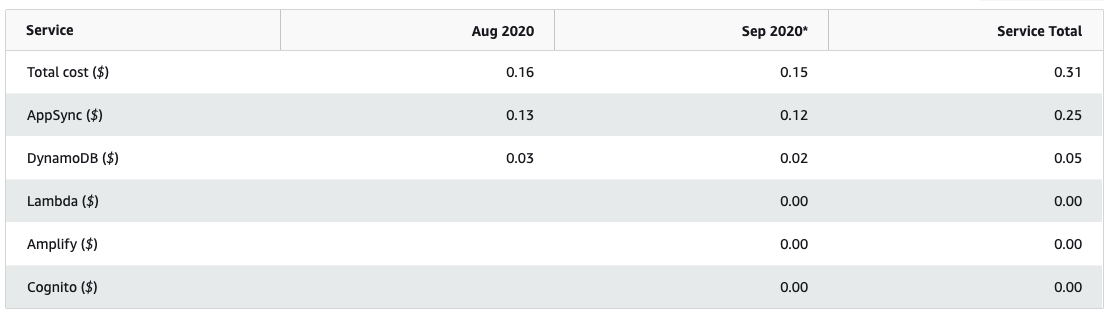
\includegraphics[width=1.0\textwidth]{50-Implementierung/Kosten.png}
    \caption{Kostenaufstellung der letzten zwei Monate}
    \label{fig:kosten}
\end{figure}
\clearpage

\subsection{Zusammenfassung}
Im Rahmen dieser Bachelorarbeit wurde die Serverless Architektur analysiert und ein funktionsfähiger Prototyp entwickelt.
Als Motivation gilt ein steigendes Interesse an Function as a Service Diensten sowie an einer schnelleren Bereitstellung von Diensten.
Die Kostenübersicht aller Cloud-Provider der Mediengruppe RTL soll vereinfacht werden und zentral aufbereitet werden.
Damit geht die Anforderung einher eine einfache und administrationsfreie Realisierung zu ermöglichen, die im besten Fall keine hohen Kosten verursacht.
Um eine qualifizierte Aussage zu einer Implementierung mit Serverless Diensten geben zu können, wurden im Voraus die wichtigsten Cloud Computing-Modelle erläutert und den Zusammenhang zu Serverless erklärt.
Im Anschluss wurde die Serverless Architektur auf ihre Eignung geprüft und bestätigt.
Die Umsetzung sollte möglichst von nur einer Person erfolgen, ohne Expertenwissen in jedem Fachgebiet zu erfordern.

Da es mehrere mögliche Ansätze zur Umsetzung gibt, ist es besonders wichtig die einzelnen Möglichkeiten zu vergleichen.
Aus diesem Grund wurden im Rahmen der Bachelorarbeit einzelne Dienste des Cloud Providers AWS untersucht und miteinander verglichen.
Nachdem die zugrundeliegende Technologie des Dienstes und der Funktionsumfang des Dienstes geprüft wurden, konnte schließlich eine Entscheidung gefällt werden.
Die einzelnen zu prüfenden Bereiche beschäftigten sich mit den Themen API, Datenbanken, Backend-Logik und Authentifizierung.
In jedem Bereich wurde ein passender Dienst ausgewählt und im weiteren Verlauf auch implementiert.
Als API wurde der AWS Dienst AppSync genutzt, der auf GraphQL basiert.
Der Dienst AWS Cognito übernimmt die Authentifizierung und Absicherung der Anwendung.
Als relationale Datenbank kommt der Dienst AWS DynamoDB zum Einsatz.
Die Backend-Logik wird mit dem Function as a Service Dienst AWS-Lambda realisiert.
Das Frontend wurde mit dem JavaScript-Framework React erstellt.
AWS Amplify dient als zentraler Dienst, um alle zuvor genannten Komponenten an zentraler Stelle konfigurieren zu können.

Das Ziel des Prototyps war es, eine funktionale Webanwendung zu erzeugen die eine Übersicht über alle aktiven AWS Accounts liefert.
Dafür musste ein Accountübergreifender Zugriff eingerichtet werden, da sich die benötigten Daten in einem anderen Account befinden als die Anwendung selbst.
Die gesammelten Daten speichert die Lambda-Funktion in eine DynamoDB-Tabelle ab.
Auf diese Daten greift das Frontend über die API zu, und erstellt mithilfe von React eine übersichtliche Tabelle aller Daten.
Da die gesamte Webanwendung im Internet erreichbar ist, wurde mit AWS Cognito eine Authentifizierung sichergestellt.
Registrierte Nutzer können die Webanwendung nutzen und auf die Daten zugreifen.

Während der Entwicklung wurde darauf geachtet eine möglichst einheitliche Programmiersprache zu verwenden.
Aufgrunddessen können andere Kollegen der Abteilung Datacenter and Clouds, ohne viel Einarbeitung, an dieser Webanwendung weiterentwickeln.
Zudem ist dank Anbindung an den Dienst GitHub eine gemeinsame Bearbeitung mühelos möglich.
Die Versionsverwaltung ermöglicht es zudem leicht Änderungen nachzuvollziehen.







